\documentclass[a4paper, twocolumn]{article}
\usepackage[pdftex, hidelinks]{hyperref}

\usepackage{bm}
\usepackage[T1]{fontenc}
\usepackage[utf8]{inputenc}
\usepackage{algorithmic}
\usepackage{algorithm}
\usepackage{amsfonts}
\usepackage{amssymb}
\usepackage{courier}
\usepackage{booktabs}
\usepackage{graphicx}
\usepackage{listings}
\usepackage{mathtools}
\usepackage{amssymb}
\lstset{basicstyle=\footnotesize\ttfamily,
breakatwhitespace = false,
breaklines = true,
keepspaces = true,
language = R,
showspaces = false,
showstringspaces = false,
belowcaptionskip = \bigskipamount,
framerule = 0.80pt,
frame = tb,
belowskip = \bigskipamount,
escapeinside={<@}{@>}}

\title{TDDE01 -- Machine Learning \\
Group 9 Laboration Report 5}
\author{{Martin Estgren \texttt{<mares480>}} \\
{Erik S. V. Jansson \texttt{<erija578>}} \\
{Sebastian Maghsoudi \texttt{<sebma654>}} \\~\\
{Linköping University (LiU), Sweden}}

\begin{document}
\pagenumbering{arabic}
    \maketitle % Generate.

    Increasing the accuracy of \emph{weather forecasts} is an important task. We propose an estimator which produces the \emph{air temperature forecast} in \emph{Sweden}, given a \emph{latitude/longitude coordinate} and also \emph{date}. Some observations by \emph{SMHI}, taken from weather stations, have been given for training our estimator.

    By using a \emph{Nadaraya–Watson regression kernel}, we can estimate the temperatures \(\bm{y'}\). This is done by taking the \emph{kernels} \(k_\sigma(\bm{x}^{(i)}, \bm{x'})\) for each \(i^{th}\) data from the training set and using it as a \emph{weight} when considering the response variable \(\bm{y}^{(i)}\). Essentially, the kernel \(k_\sigma(\bm{x}^{(i)}, \bm{x'})\) will reduce \(\bm{y}^{(i)}\)'s significance in the \emph{total contribution} by giving less weight when the \(\bm{x^{(i)}}\) and \(\bm{x'}\) are further away (in some measure).

    We have used a \emph{Gaussian Radial Basis Function} as our \emph{kernel}, which is defined in Equation~\ref{eq:grbf} below. Note the parameter \(\sigma\), which can be considered as the \emph{spread} or \emph{width} of the kernel, and also \(\bm{x^{(i)}} - \bm{x'}\) which is the \emph{distance function}; giving our kernel the property of a \emph{similarity function} (because of \(e^{(\cdots)}\)).

    By using \(k_\sigma(\bm{x}^{(i)}, \bm{x'})\) in \emph{Nadaraya–Watson's} \(\bm{y'}\) estimator, shown in Equation~\ref{eq:nadaraya_watson}, we are essentially \emph{weighing} how important the contributions from \(\bm{y}^{(i)}\) are to \(\bm{y'}\), because \emph{similar} \(\bm{x}^{(i)}\) will give higher \(k_\sigma\).

    \begin{equation} \label{eq:grbf}
    k_\sigma(\bm{x}, \bm{x'}) = \mathrm{exp}\bigg(\frac{- \, {\left\Vert(\bm{x} - \bm{x'}) \right\Vert}^2}
    {2\sigma^2 \; \{\sigma \approx h\}}\bigg)
    \end{equation}

    \begin{equation} \label{eq:nadaraya_watson}
    \bm{y'}(\bm{x}, \bm{x'}) = \frac{\sum_n{\bm{y}^{(i)}k_\sigma(\bm{x}^{(i)}, \bm{x'})}}
    {\sum_n{k_\sigma(\bm{x}^{(i)}, \bm{x'})}}
    \end{equation}

    \lstinputlisting[firstline=23,lastline=25]{../share/script.r}

    We now describe the functions which were used to determine the distance/similarity for the kernels.

    Below follows the applied \emph{distance functions}, which give the measured distance between a pair of \emph{locations}, \emph{times of the day}, and also \emph{dates of year}. These distance and kernel functions can be found in Listing~\ref{lst:script}, where they follow similarly as described.

    \begin{equation*} \label{eq:location}
    d_l = r\, \mathrm{hav}^{-1}(h),\; \mathrm{hav}(\varphi) = \frac{1 - \cos\varphi}{2}
    \end{equation*}
    
    \lstinputlisting[firstline=28,lastline=32]{../share/script.r}
    
    \begin{equation*} \label{eq:time}
    d_t = \begin{cases}
    |x - y| & |x - y| < (x + y) \bmod 24\\
    (x + y) \bmod 24 & |x - y| \geq (x + y) \bmod 24
    \end{cases}
    \end{equation*}

   \lstinputlisting[firstline=45,lastline=51]{../share/script.r}

    \begin{equation*} \label{eq:day}
    d_d = \begin{cases}
    |x - y| & |x - y| < (x + y) \bmod 365\\
    (x + y) \bmod 365 & |x - y| \geq (x + y) \bmod 365
    \end{cases}
    \end{equation*}

   \lstinputlisting[firstline=35,lastline=42]{../share/script.r}

    Finally, we have the \emph{three different kernels} which contribute in unison to the final \emph{forecast kernel}. Each of these use Equation~\ref{eq:grbf} with their respective \emph{distance functions} and also \emph{kernel width} \(h\) (\(\sigma\) here).

    \lstinputlisting[firstline=67,lastline=70]{../share/script.r}

	An obvious question the reader has by now is:\newline~\newline\textit{What values should be assigned to \(2\sigma^2\)?}\newline~\newline If said reader does not wonder about this, said reader needs to be more intellectually involved in this papers reasoning in the future. However, the answer to the question has to do with the scale of the range of values that the distance can have. One could assign 1 to as a weight, and it might be sufficient, especially if the values are not very large for relatively close observations. This means it is completely related to the context. When in the the context of physical distance it is reasonable to use 1000000 as \textit{h} since if the point of interest is only a few km away from an already existing observation, the kernel value will return close to 0 values. For date and time, the values already seems to be good enough and only needs to be modified with very small factors. Date uses 3 for \textit{h} and time uses 2. The intuition seems to be confirmed when observing the result from the kernels presented in Figures~\ref{fig:time}, \ref{fig:date} and \ref{fig:dist}, which are described in detail.

    The date and time formats for the data set required pre-processing before they could be used in the above mentioned functions. This is done with:
    \lstinputlisting[firstline=104,lastline=108]{../share/script.r}

    The plots in Figure~\ref{fig:date} shows the date-kernel distance for each of the observations. It's harder to detect the trend in the date feature but we can observe a spike each year. For the purpose of processing, all years are set to 2016.
    \begin{figure}[H]
    \centering
        \caption{Date distance plot for the observations}\label{fig:date}
	    \begin{minipage}[]{0.32\textwidth}
	    	\includegraphics[width=\textwidth]{share/1_date.png}
	    \end{minipage}
    \end{figure}

    The plots in Figures~\ref{fig:dist} shows the longitude/latitude-kernel distance for each of the observations. The data is ordered by station number. As expected we can observe a specific group of stations closer with a higher kernel value that others. Given that there's a relation between the station number and location this is expected.
    \begin{figure}[H]
    \centering
        \caption{Station distance plot for the observations}\label{fig:dist}
	    \begin{minipage}[]{0.32\textwidth}
	    	\includegraphics[width=\textwidth]{share/1_dist.png}
	    \end{minipage}
    \end{figure}

    The plots in Figures~\ref{fig:time} shows the time-kernel distance for each of the observations.  

    \begin{figure}[H]
    \centering
    \caption{Distance plot (time of day) for the observations (Ordered by time of day) \label{fig:time}}
	    \begin{minipage}[]{0.2\textwidth}
	    	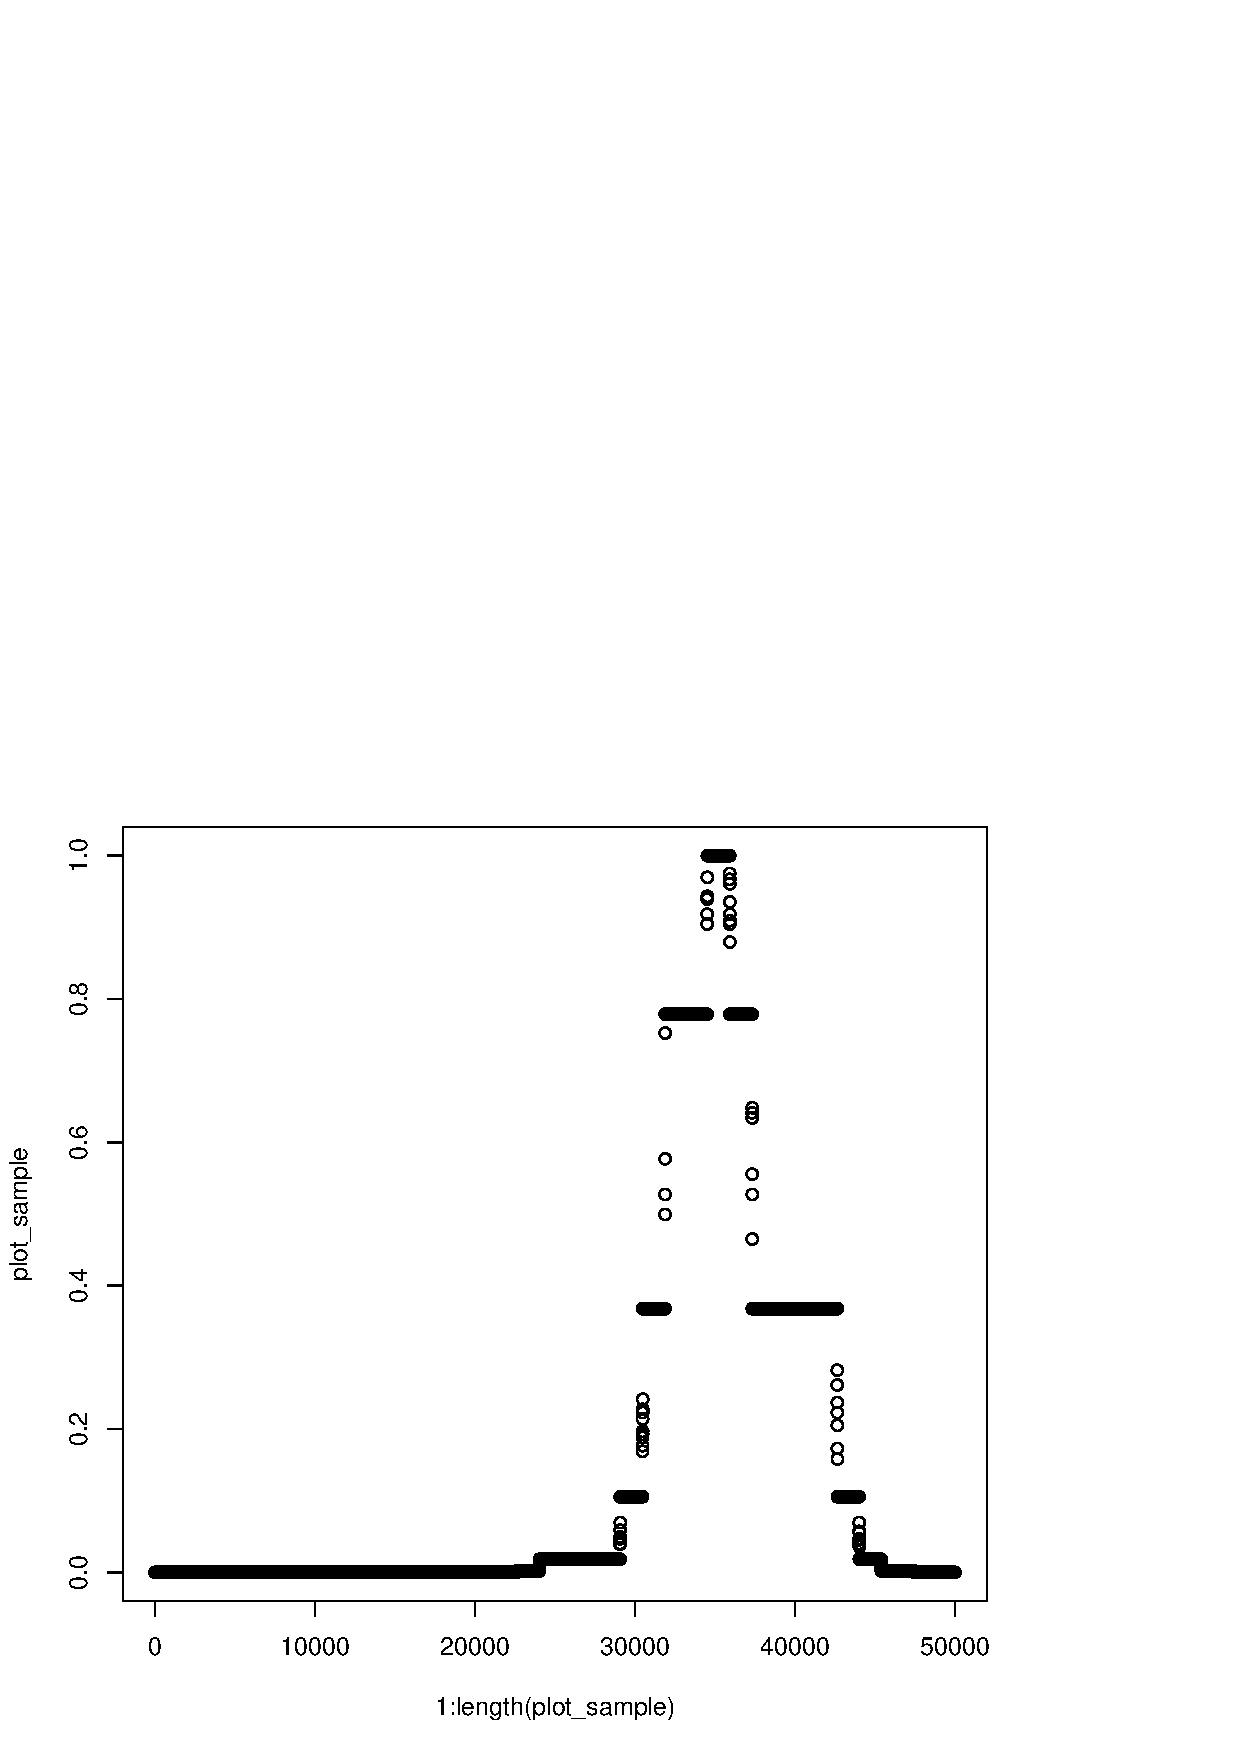
\includegraphics[width=\textwidth]{share/1_time.png}
	    \end{minipage}
	    \begin{minipage}[]{0.2\textwidth}
	    	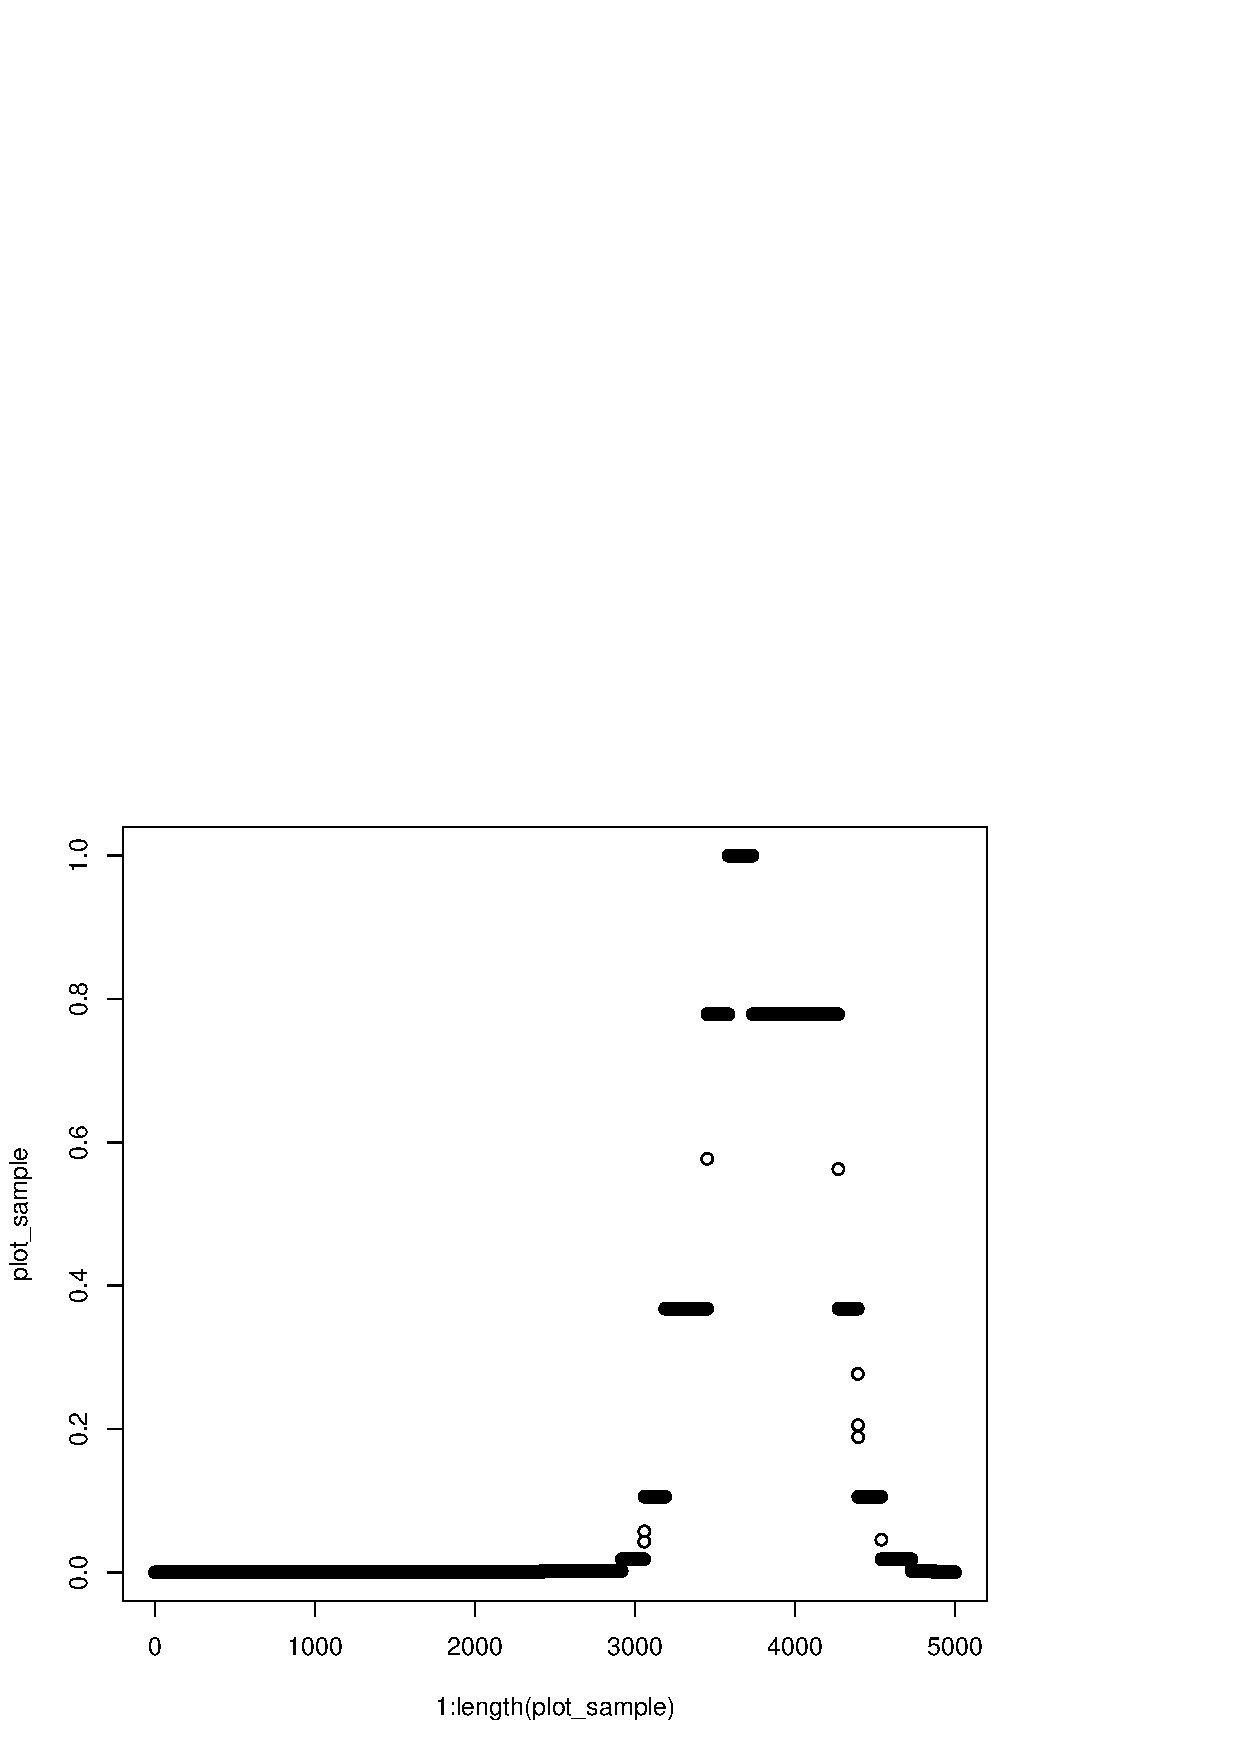
\includegraphics[width=\textwidth]{share/2_time.png}
	    \end{minipage}
	    \begin{minipage}[]{0.2\textwidth}
	    	\includegraphics[width=\textwidth]{share/3_time.png}
	    \end{minipage}
	    \begin{minipage}[]{0.2\textwidth}
	    	\includegraphics[width=\textwidth]{share/4_time.png}
	    \end{minipage}
	    \begin{minipage}[]{0.2\textwidth}
	   		 \includegraphics[width=\textwidth]{share/5_time.png}
	    \end{minipage}
	    \begin{minipage}[]{0.2\textwidth}
	    	\includegraphics[width=\textwidth]{share/6_time.png}
	    \end{minipage}
	    \begin{minipage}[]{0.2\textwidth}
	    	\includegraphics[width=\textwidth]{share/7_time.png}
	    \end{minipage}
	    \begin{minipage}[]{0.2\textwidth}
	   		 \includegraphics[width=\textwidth]{share/8_time.png}
	    \end{minipage}
	    \begin{minipage}[]{0.2\textwidth}
	    	\includegraphics[width=\textwidth]{share/9_time.png}
	    \end{minipage}
	    \begin{minipage}[]{0.2\textwidth}
	    	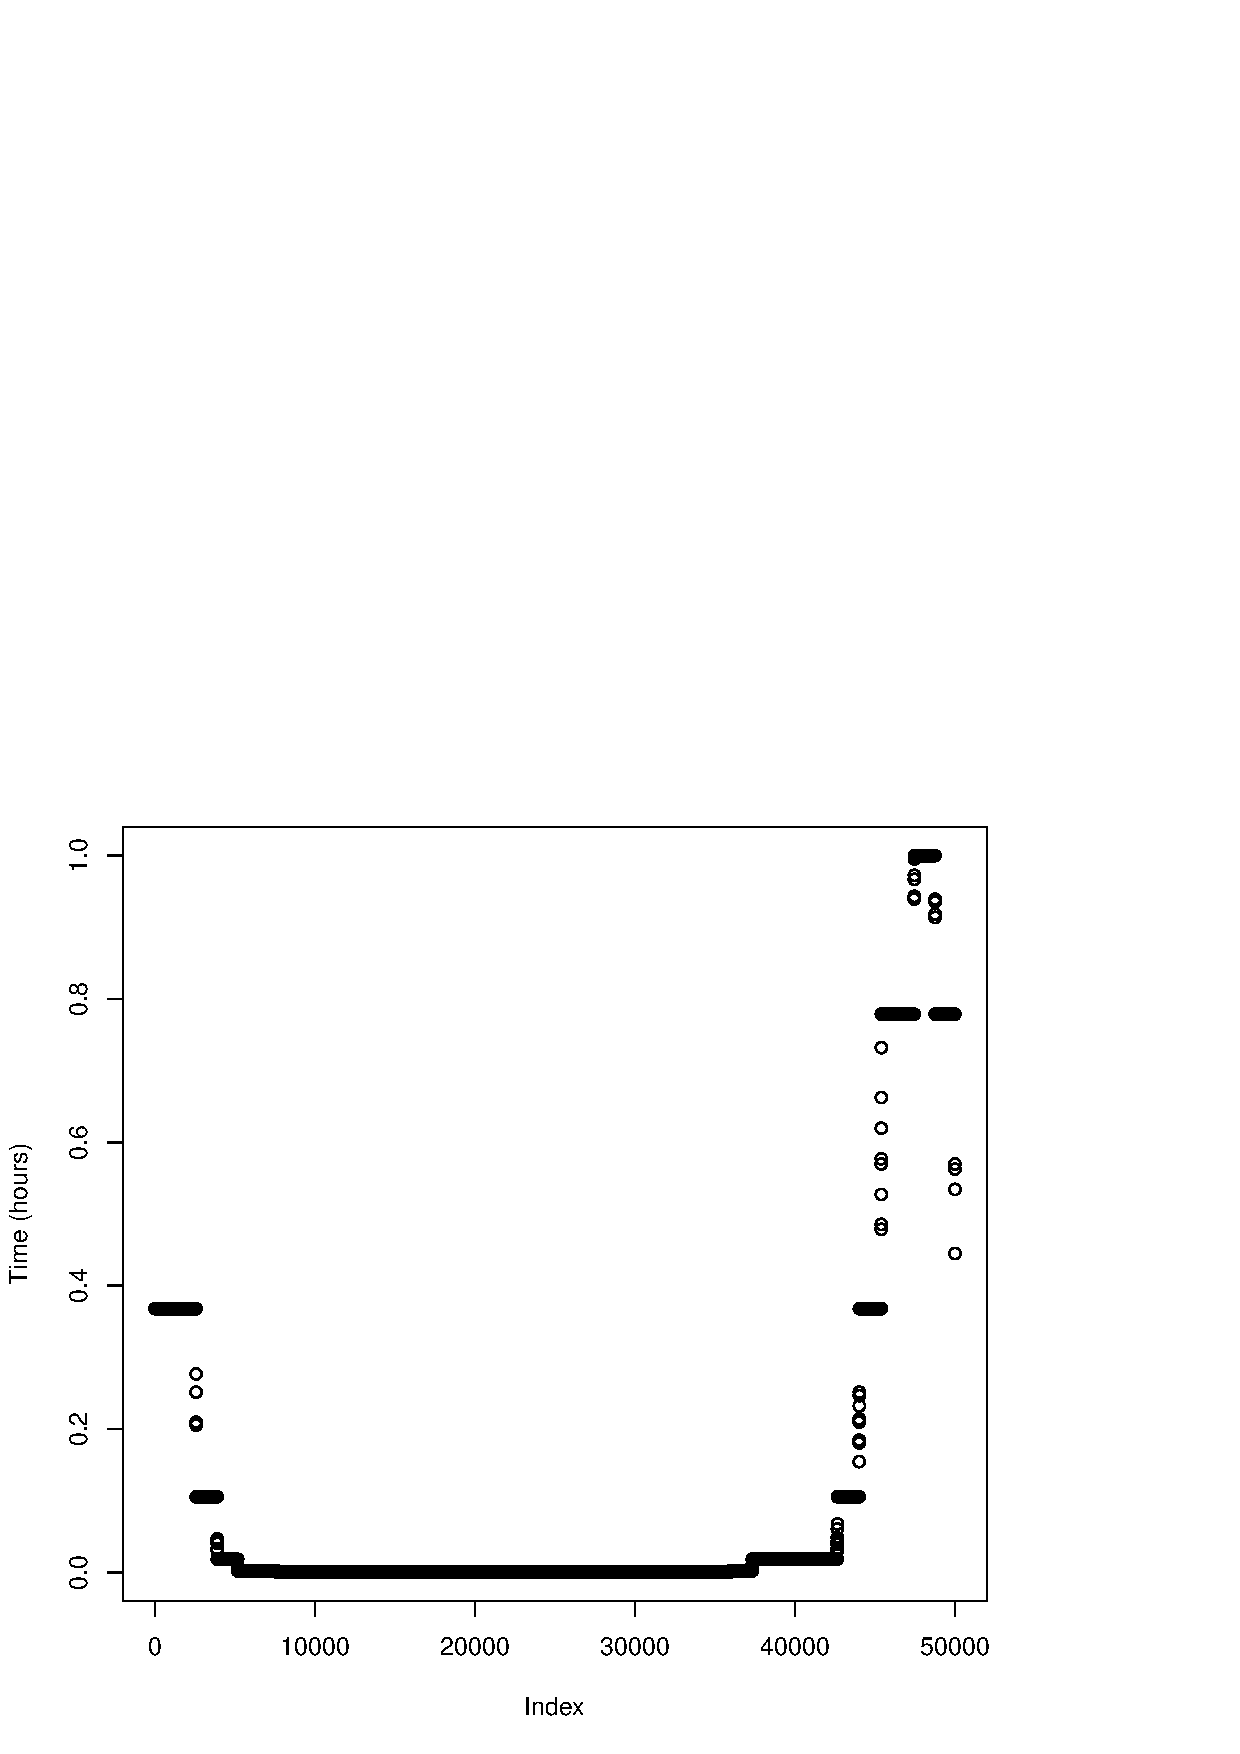
\includegraphics[width=\textwidth]{share/10_time.png}
	    \end{minipage}
	    \begin{minipage}[]{0.4\textwidth}
	    	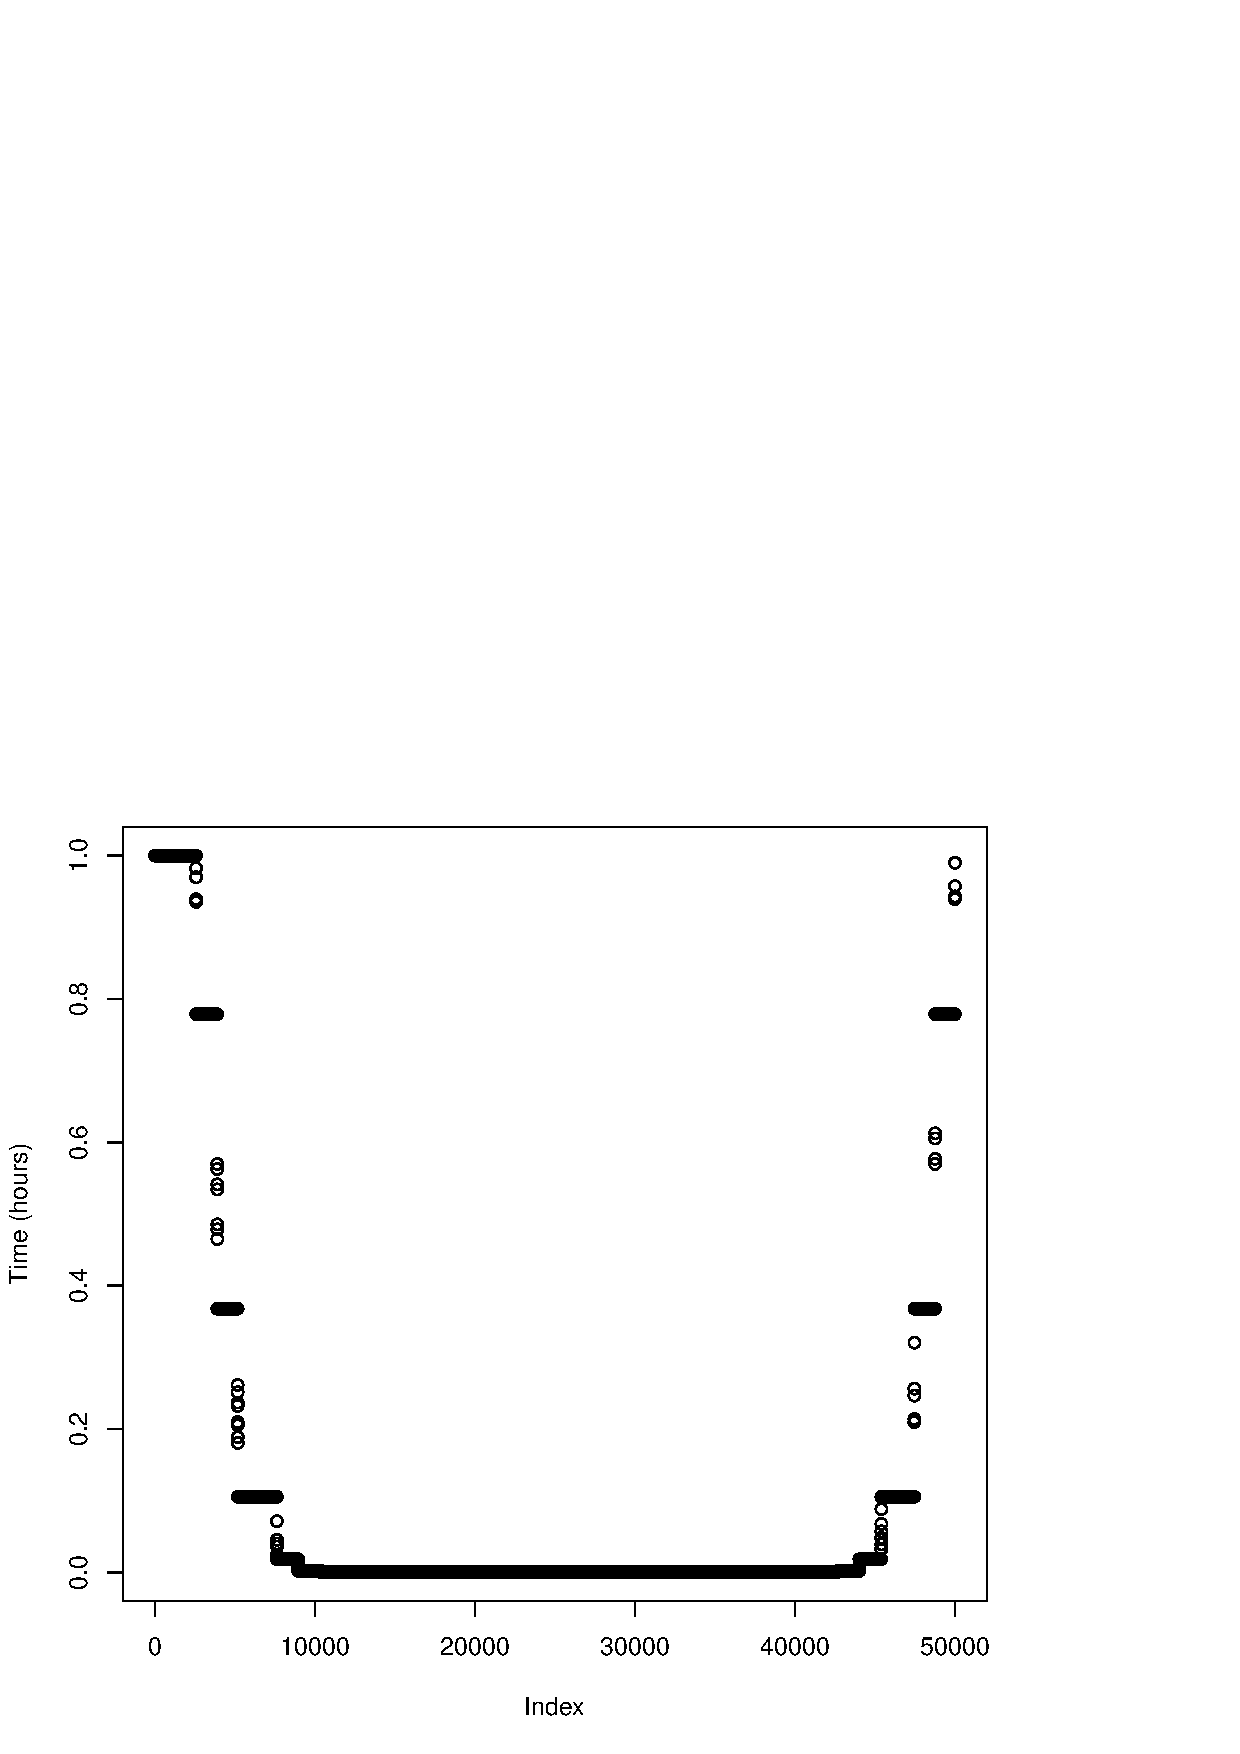
\includegraphics[width=\textwidth]{share/11_time.png}
	    \end{minipage}
    \end{figure}
	The figures would indicate that the close a given data sample (time of day) is to the observation the greater the value of the kernel. In the last couple of figures we can observe how the kernel value loops around the clock, as would be expected.



    The plots in Figures~\ref{fig:result} shows the predicted \textit{air temperature} for each of the observations. 
    \begin{figure}[H]
    \centering
        \caption{Predicted temperature for the day 2013-04-12 in the interval 04:00-24:00 (ordered by hour)}\label{fig:result}
	    \begin{minipage}[]{0.4\textwidth}
	    	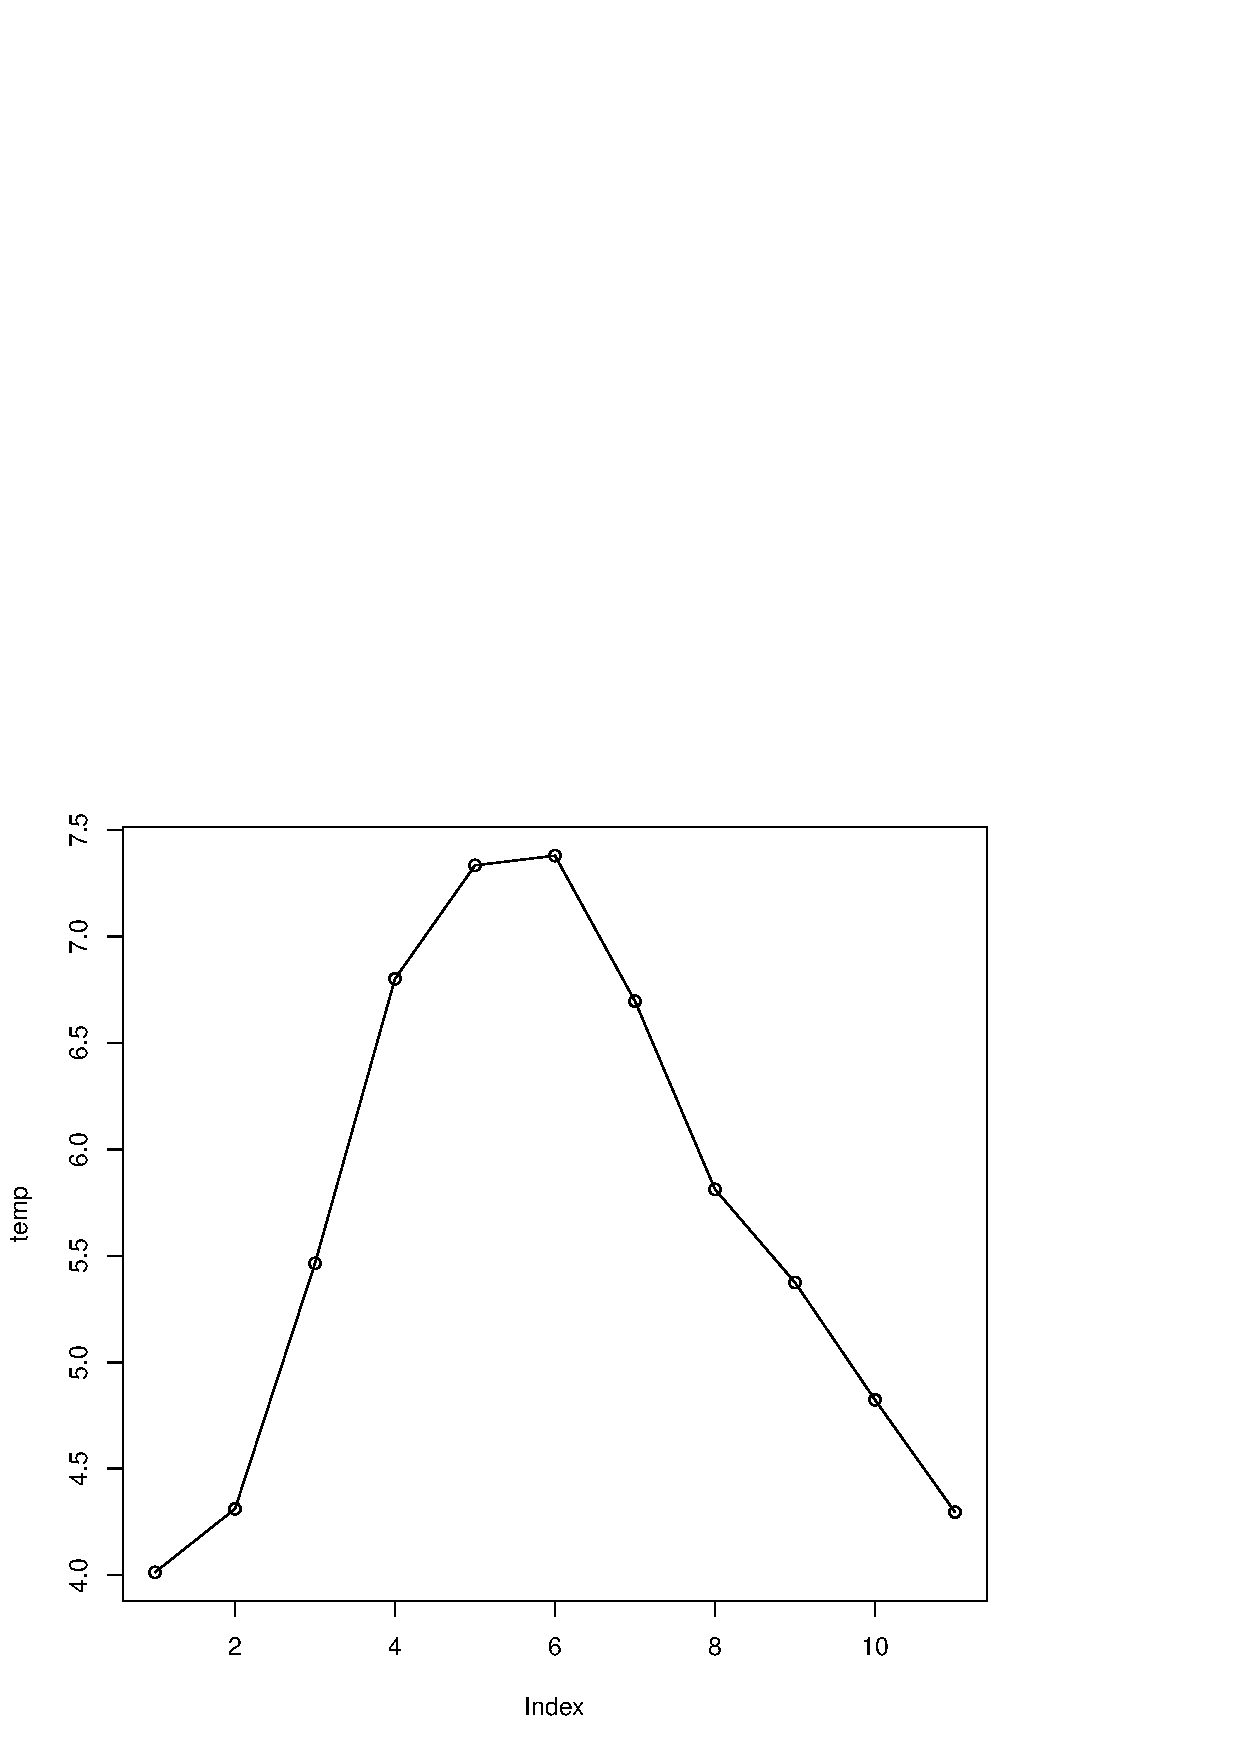
\includegraphics[width=\textwidth]{share/result.png}
	    \end{minipage}
    \end{figure}

	In Figure~\ref{fig:result} the observer might wonder the following question: \textit{Why are the temperatures this low?}\newline
    The obvious answer is that the point of interest is in Sweden. But the actual answer might be that, since the kernel feature are independent from one another, two "good" values might counter one "bad" value. Meaning that two of the kernels might return very high values since they almost completely match with the point of interest. One value however might be very small, e.g. the date is completely in the wrong season. This issue will pull the predicted temperature to the sample average. However, there is a solution to this problem. In order to avoid that irrelevant observations affects the result, one might exclude such observation. In truth could only include a number of observations (100) that are reasonably close to the point of interest. This will make the result much more reasonable in this aspect. There is however a limit to where the data stops being reasonable because of spikes in temperature change. This happens because to few observations are used.

    \begin{figure}[H]
    \centering
    \caption{Predicted temperature for the day 2013-07-12 in the interval 04:00-24:00 (ordered by hour)\label{fig:bad_result}}
	    \begin{minipage}[]{0.4\textwidth}
	    	\includegraphics[width=\textwidth]{share/bad_result.png}
	    \end{minipage}
    \end{figure}
	In Figure~\ref{fig:bad_result} the observations for the date 2013-07-12 can be observed. As described above, the mean temperature of the year means that even in one of the warmest periods where the temperature is expected to be close to \(20^\circ \) we get degrees in the ones of digits.

    \section*{Contributions}

    \begin{itemize}
    	\item{\textbf{Martin Estgren:} Provided the all the figures and code listings, also wrote some of the result analysis.}
        \item{\textbf{Erik S. V. Jansson:} Gave a general introduction to the theory relevant in this assignment, such as the \emph{gaussian kernel} and \emph{Nadaraya–Watson kernel regression equations}.}
    	\item{\textbf{Sebastian Maghsoudi:} Answered questions specified in the assignment,(width and odd temperatures).}
    \end{itemize}

    \nocite{*} % No warnings.
    \bibliographystyle{alpha}
    \bibliography{report}
    \onecolumn \appendix
    \section*{Appendix}
 	\lstinputlisting[caption={Script for Assignment},label={lst:script}]{../share/script.r}


    \end{document}
